\subsection*{Explicación}
Al analizar el comportamiento del Tlatch observamos que este invierte los valores de q y qn cuando t=1 y c=1.\\
En la implementación añadí un delay y un caso base para que no todos los valores de q y qn sean desconocidos al realizar a simulación. 

\subsection*{Tabla de verdad}
\begin{figure}[h]
    \centering
    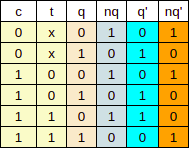
\includegraphics{fotos/TruthTable/arki-lab2-TT_tlatch.png}
\end{figure}

\subsection*{Mapa de Karnaugh}
\begin{figure}[h]
    \centering
    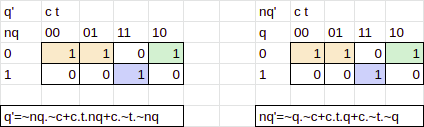
\includegraphics[scale=0.8]{fotos/kmaps/arki-lab2-kmap_tlatch.png}
\end{figure}
%\subsection*{Ecuaciones booleanas}

\newpage
\subsection*{Resultados}
\begin{figure}[htbp]
    \centering
    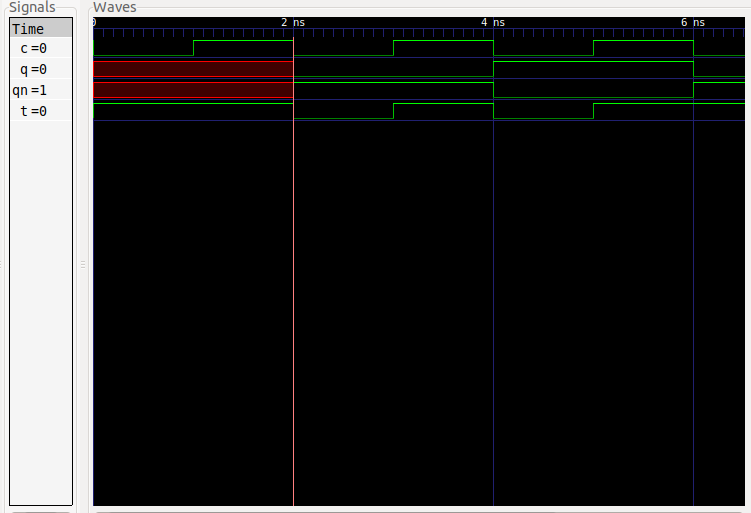
\includegraphics[scale=0.5]{fotos/resultados/arki-lab2-R_tlatch.png}
\end{figure}